\section{6-11 Notes}

I am now using Stan instead of PyMC.  Things are an order of magnitude faster, and chains doesn't seem to get stuck.

\subsection{Fitting Model to Simulated Data}
\begin{itemize}
\item Can recover $B^a,B^b,B^c$ (mode of posterior for those parameters is that used to simulate the data) when simulation is done with \emph{no} noise at all - all $\phi$'s 0 when doing simulation.  
\item If during simulation, $\phi^a,\phi^b,\phi^c$ are zero, but $\phi^{noise}$ is nonzero, the chain doesn't move around.
\item If during simulation, $\phi^a,\phi^b,\phi^c$ are nonzero, but $\phi^{noise}$ is zero, $B_b$ is slightly off.
\item For case when all $\phi$ parameters are nonzero, don't think I ran chain long enough yet to conclude anything.
\end{itemize}

\subsection{Fitting Model to Real Data}
\begin{itemize}
\item Only looked at 2 covariates for now (function level before treatment, age)
\item Features normalized to have 0 mean, unit variance.
\item Calculated $\mu_{pop}^a, \mu_{pop}^b, \mu_{pop}^c$ by, for each patient, doing curve fitting to get a least squares estimate of their $a,b,c$ parameters.  Omitted from dataset patients with less than 7 time point values.
\item Set $c^a,c^b,c^c$ all equal to 1.0 (the std of the normal priors for $B^a,B^b,B^c$).
\item Had to set $\lambda^a,\lambda^b,\lambda^c$ to be quite large(10) to force $\phi^a,\phi^b,\phi^c$ to be not too big.  If I didn't do this, each $a_i,b_i,c_i$ would come from a very diffuse distribution, in which case the model would not be sensitive to the values of the linear coefficients $B^a,B^b,B^c$, causing them to vary wildly (jump between -10000 and +10000)
\end{itemize}

\subsection{What I plotted}
\begin{itemize}
\item Posterior Distribution of the $B^a,B^b,B^c$.  Since I looked at 2 covariates, these parameters are length 2 vectors.  I plotted $B^a[0]$ and $B^a[1]$ on the same plot, same for $B^b,B^c$.  The component corresponding to the pre-treatment function level is red.  The component corresponding to age is green.
\item I also plot, for each of the 2 covariates, scatter plot of the covariate vs. the $a,b,c$ parameters as obtained by curve fitting, as well as the initial "drop" relative to pre-treatment function value(this is a function of $a$ and $b$.
\item I also include plots of the beta and gamma distributions for various values of dispersion parameters so we have a grasp of what distributions with particular dispersion parameters look like.
\end{itemize}

\begin{figure}
\begin{subfigure}{
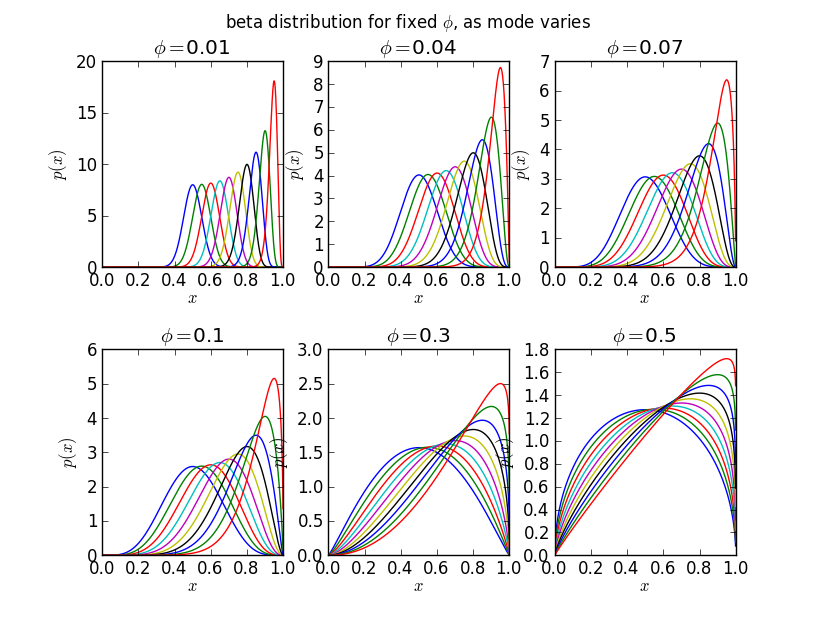
\includegraphics[width=.45\linewidth,height=0.3\textheight]{/Users/glareprotector/Documents/lab/glare/tex_files/sections/analyze_bias/files/beta_phi.png}}
\end{subfigure}
\begin{subfigure}{
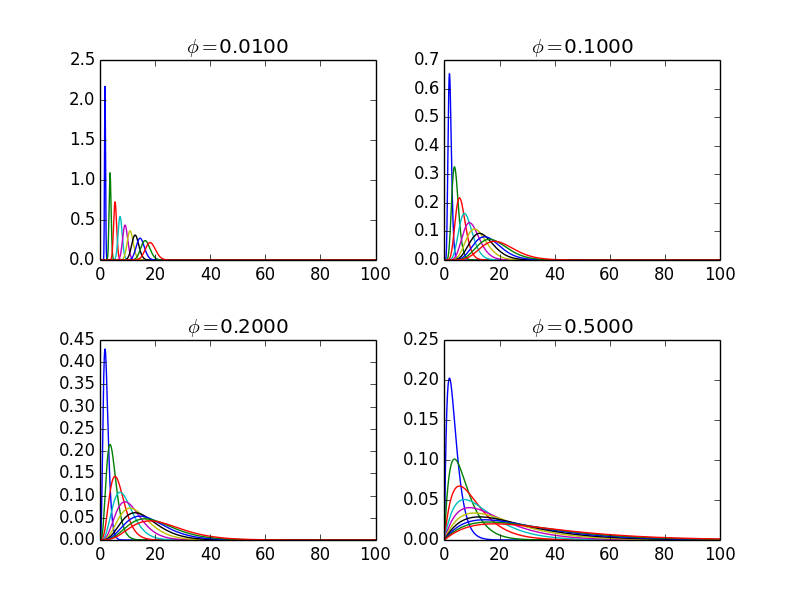
\includegraphics[width=.45\linewidth,height=0.3\textheight]{/Users/glareprotector/Documents/lab/glare/tex_files/sections/gamma_distribution/files/gamma_dist.png}}
\end{subfigure}
\caption{Beta and Gamma distributions for different values of respective $\phi$'s}
\end{figure}


\begin{figure}
\centering
\begin{subfigure}{
  \includegraphics[width=.45\linewidth,height=0.3\textheight]{/Users/glareprotector/Documents/lab/glare/prostate_code/files_for_rstan/sexual_function/surgery/B_abc_hist.png}}
\end{subfigure}
\begin{subfigure}{
  \includegraphics[width=.45\linewidth,height=0.3\textheight]{/Users/glareprotector/Documents/lab/glare/prostate_code/files_for_rstan/sexual_function/surgery/B_phi_hist.png}}
\end{subfigure}
\begin{subfigure}{
  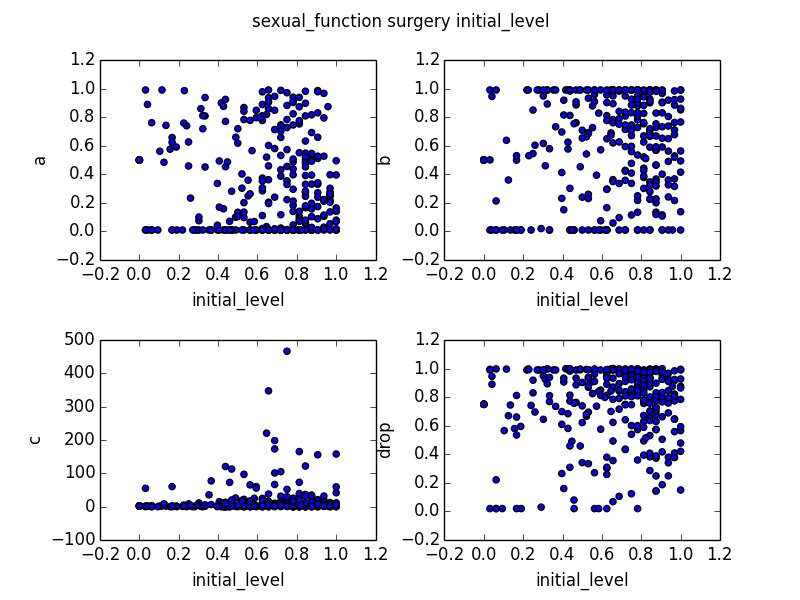
\includegraphics[width=.45\linewidth,height=0.3\textheight]{/Users/glareprotector/Documents/lab/glare/tex_files/sections/exploratory_with_abc/files/attribute_vs_curve_parameters/sexual_function_surgery_initial_level.png}}
\end{subfigure}
\begin{subfigure}{
  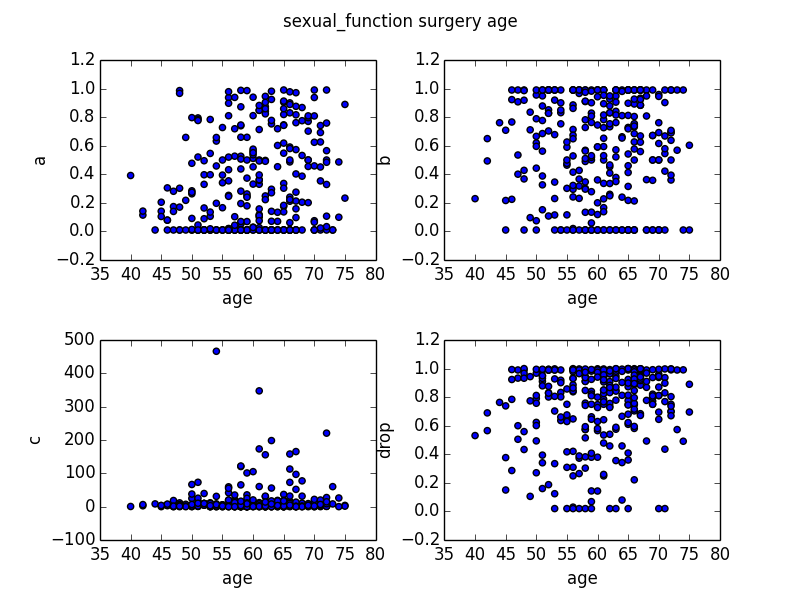
\includegraphics[width=.45\linewidth,height=0.3\textheight]{/Users/glareprotector/Documents/lab/glare/tex_files/sections/exploratory_with_abc/files/attribute_vs_curve_parameters/sexual_function_surgery_age.png}}
\end{subfigure}
\caption{Sexual Function / Surgery}
\end{figure}

\begin{figure}
\centering
\begin{subfigure}{
  \includegraphics[width=.45\linewidth,height=0.3\textheight]{/Users/glareprotector/Documents/lab/glare/prostate_code/files_for_rstan/sexual_function/radiation/B_abc_hist.png}}
\end{subfigure}
\begin{subfigure}{
  \includegraphics[width=.45\linewidth,height=0.3\textheight]{/Users/glareprotector/Documents/lab/glare/prostate_code/files_for_rstan/sexual_function/radiation/B_phi_hist.png}}
\end{subfigure}
\begin{subfigure}{
  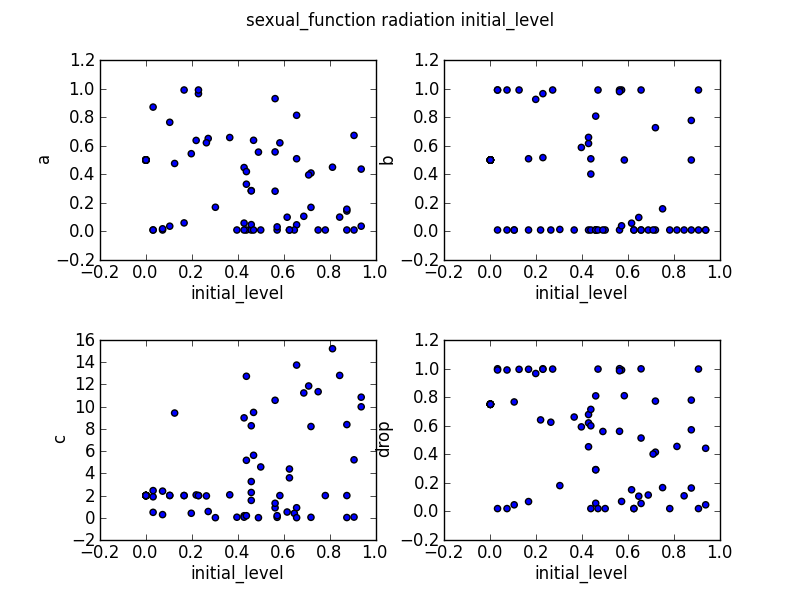
\includegraphics[width=.45\linewidth,height=0.3\textheight]{/Users/glareprotector/Documents/lab/glare/tex_files/sections/exploratory_with_abc/files/attribute_vs_curve_parameters/sexual_function_radiation_initial_level.png}}
\end{subfigure}
\begin{subfigure}{
  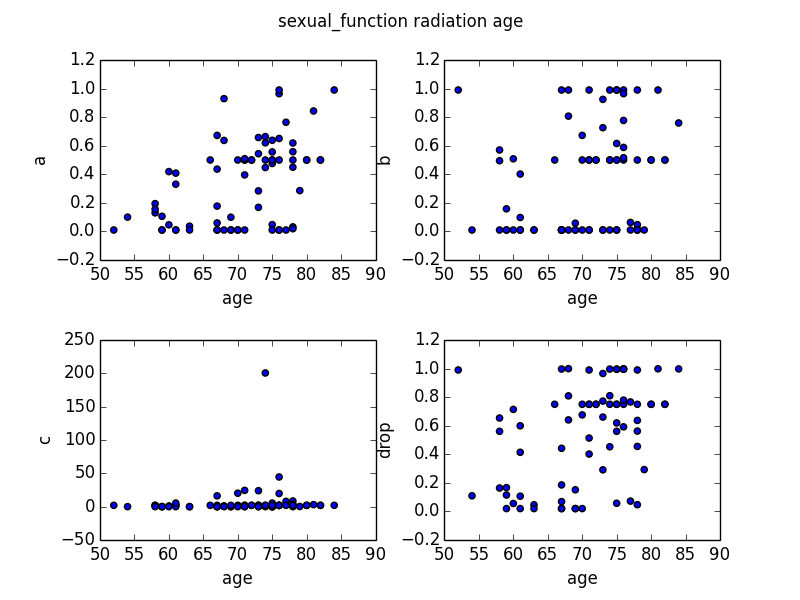
\includegraphics[width=.45\linewidth,height=0.3\textheight]{/Users/glareprotector/Documents/lab/glare/tex_files/sections/exploratory_with_abc/files/attribute_vs_curve_parameters/sexual_function_radiation_age.png}}
\end{subfigure}
\caption{Sexual Function / Radiation}
\end{figure}

\begin{figure}
\centering
\begin{subfigure}{
  \includegraphics[width=.45\linewidth,height=0.3\textheight]{/Users/glareprotector/Documents/lab/glare/prostate_code/files_for_rstan/sexual_function/brachytherapy/B_abc_hist.png}}
\end{subfigure}
\begin{subfigure}{
  \includegraphics[width=.45\linewidth,height=0.3\textheight]{/Users/glareprotector/Documents/lab/glare/prostate_code/files_for_rstan/sexual_function/brachytherapy/B_phi_hist.png}}
\end{subfigure}
\begin{subfigure}{
  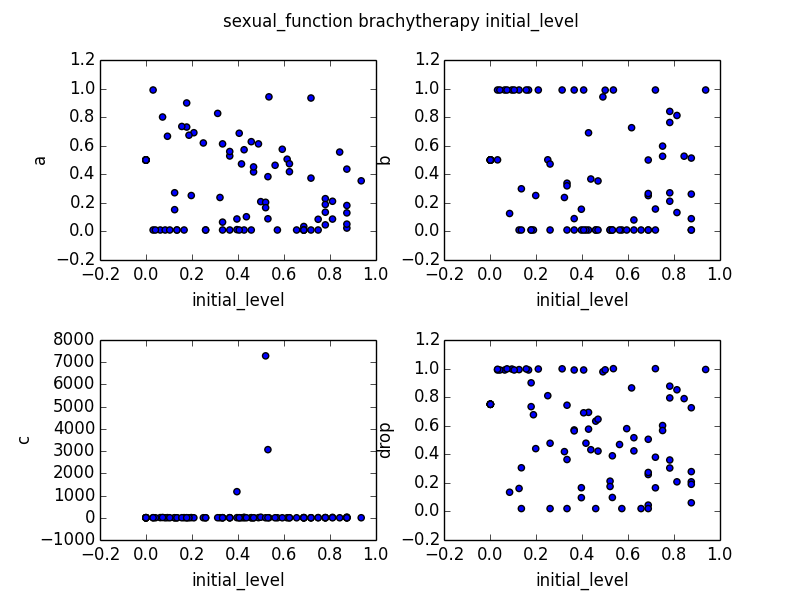
\includegraphics[width=.45\linewidth,height=0.3\textheight]{/Users/glareprotector/Documents/lab/glare/tex_files/sections/exploratory_with_abc/files/attribute_vs_curve_parameters/sexual_function_brachytherapy_initial_level.png}}
\end{subfigure}
\begin{subfigure}{
  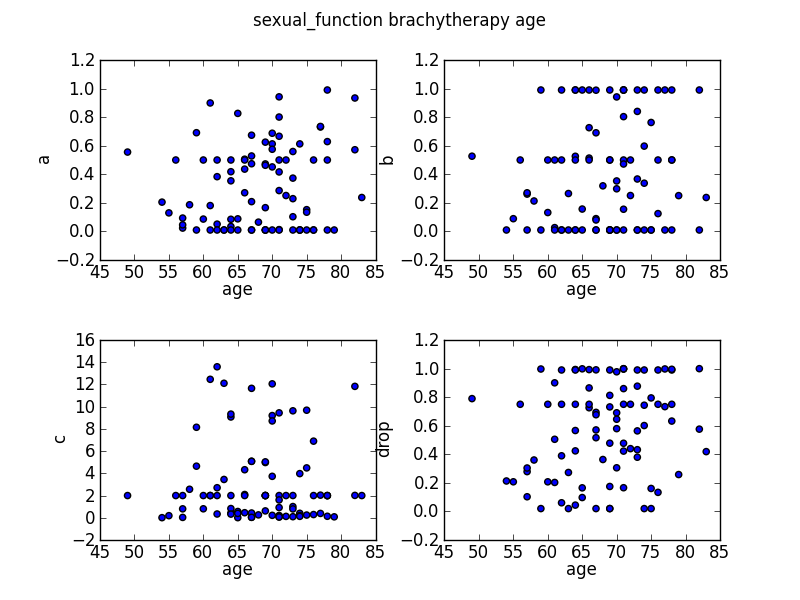
\includegraphics[width=.45\linewidth,height=0.3\textheight]{/Users/glareprotector/Documents/lab/glare/tex_files/sections/exploratory_with_abc/files/attribute_vs_curve_parameters/sexual_function_brachytherapy_age.png}}
\end{subfigure}
\caption{Sexual Function / Brachytherapy}
\end{figure}

\begin{figure}
\centering
\begin{subfigure}{
  \includegraphics[width=.45\linewidth,height=0.3\textheight]{/Users/glareprotector/Documents/lab/glare/prostate_code/files_for_rstan/urinary_function/surgery/B_abc_hist.png}}
\end{subfigure}
\begin{subfigure}{
  \includegraphics[width=.45\linewidth,height=0.3\textheight]{/Users/glareprotector/Documents/lab/glare/prostate_code/files_for_rstan/urinary_function/surgery/B_phi_hist.png}}
\end{subfigure}
\begin{subfigure}{
  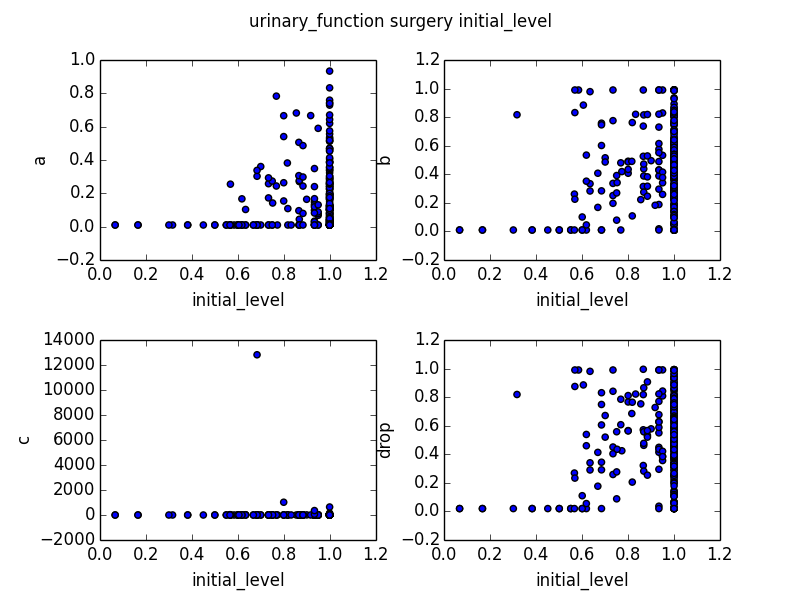
\includegraphics[width=.45\linewidth,height=0.3\textheight]{/Users/glareprotector/Documents/lab/glare/tex_files/sections/exploratory_with_abc/files/attribute_vs_curve_parameters/urinary_function_surgery_initial_level.png}}
\end{subfigure}
\begin{subfigure}{
  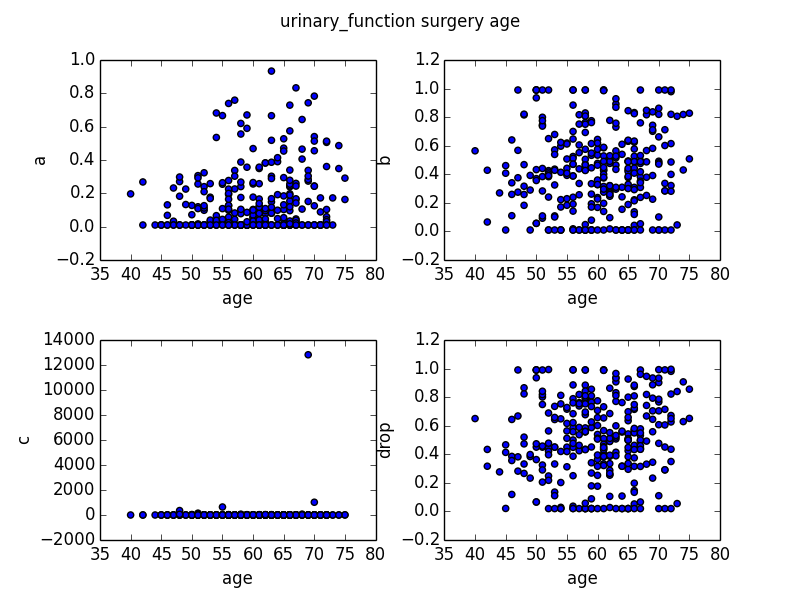
\includegraphics[width=.45\linewidth,height=0.3\textheight]{/Users/glareprotector/Documents/lab/glare/tex_files/sections/exploratory_with_abc/files/attribute_vs_curve_parameters/urinary_function_surgery_age.png}}
\end{subfigure}
\caption{Urinary Function / Surgery}
\end{figure}

\begin{figure}
\centering
\begin{subfigure}{
  \includegraphics[width=.45\linewidth,height=0.3\textheight]{/Users/glareprotector/Documents/lab/glare/prostate_code/files_for_rstan/urinary_function/radiation/B_abc_hist.png}}
\end{subfigure}
\begin{subfigure}{
  \includegraphics[width=.45\linewidth,height=0.3\textheight]{/Users/glareprotector/Documents/lab/glare/prostate_code/files_for_rstan/urinary_function/radiation/B_phi_hist.png}}
\end{subfigure}
\begin{subfigure}{
  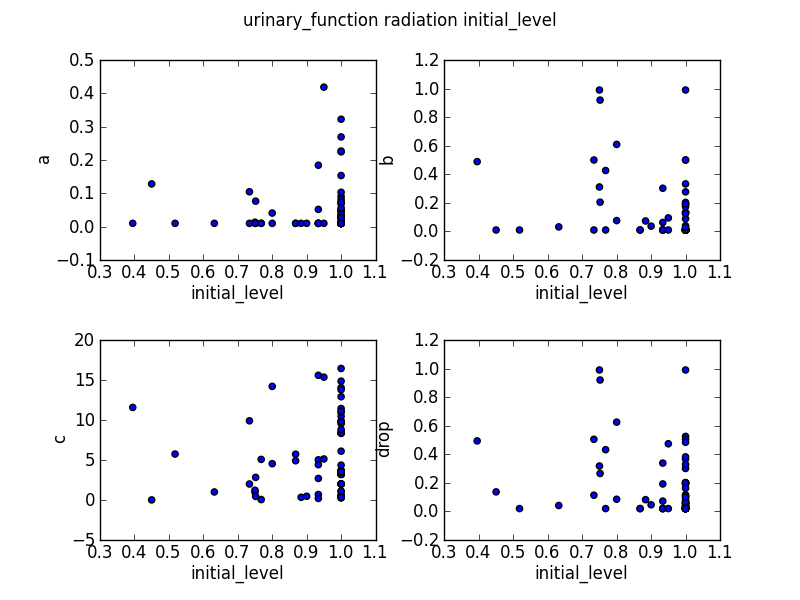
\includegraphics[width=.45\linewidth,height=0.3\textheight]{/Users/glareprotector/Documents/lab/glare/tex_files/sections/exploratory_with_abc/files/attribute_vs_curve_parameters/urinary_function_radiation_initial_level.png}}
\end{subfigure}
\begin{subfigure}{
  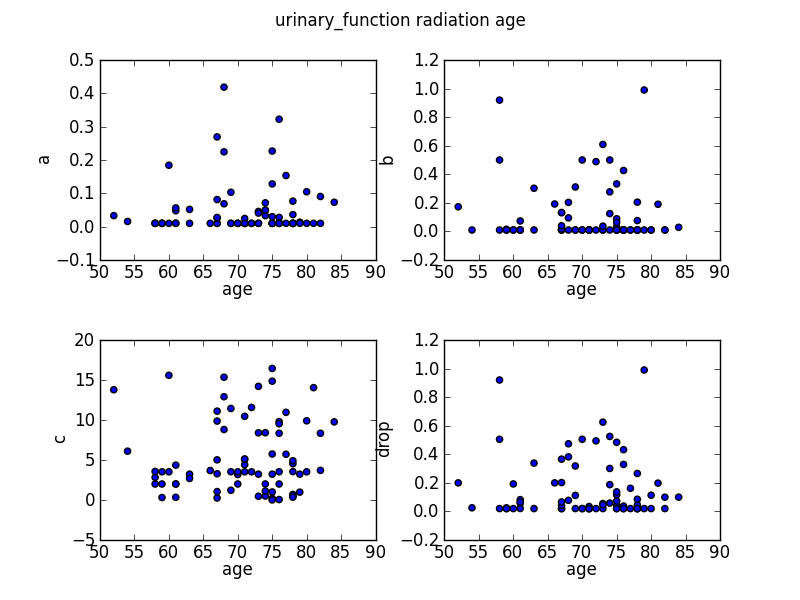
\includegraphics[width=.45\linewidth,height=0.3\textheight]{/Users/glareprotector/Documents/lab/glare/tex_files/sections/exploratory_with_abc/files/attribute_vs_curve_parameters/urinary_function_radiation_age.png}}
\end{subfigure}
\caption{Urinary Function / Radiation}
\end{figure}

\begin{figure}
\centering
\begin{subfigure}{
  \includegraphics[width=.45\linewidth,height=0.3\textheight]{/Users/glareprotector/Documents/lab/glare/prostate_code/files_for_rstan/urinary_function/brachytherapy/B_abc_hist.png}}
\end{subfigure}
\begin{subfigure}{
  \includegraphics[width=.45\linewidth,height=0.3\textheight]{/Users/glareprotector/Documents/lab/glare/prostate_code/files_for_rstan/urinary_function/brachytherapy/B_phi_hist.png}}
\end{subfigure}
\begin{subfigure}{
  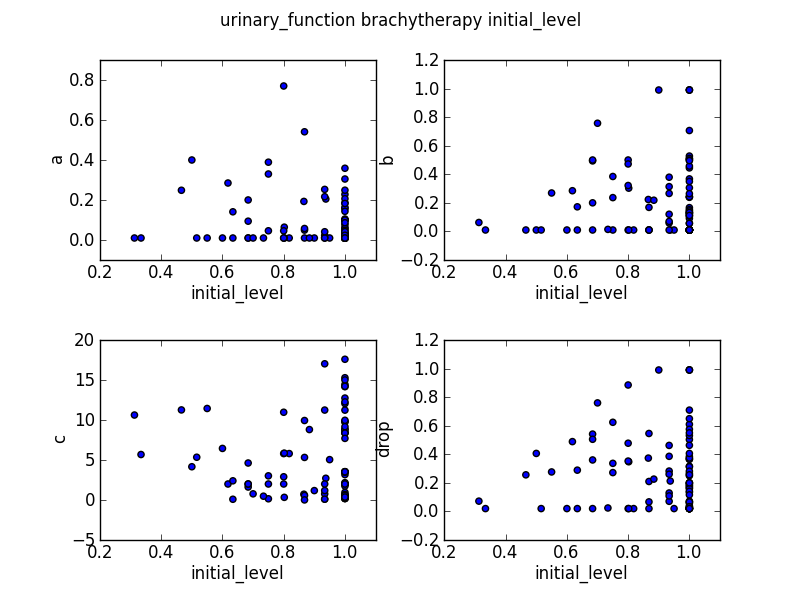
\includegraphics[width=.45\linewidth,height=0.3\textheight]{/Users/glareprotector/Documents/lab/glare/tex_files/sections/exploratory_with_abc/files/attribute_vs_curve_parameters/urinary_function_brachytherapy_initial_level.png}}
\end{subfigure}
\begin{subfigure}{
  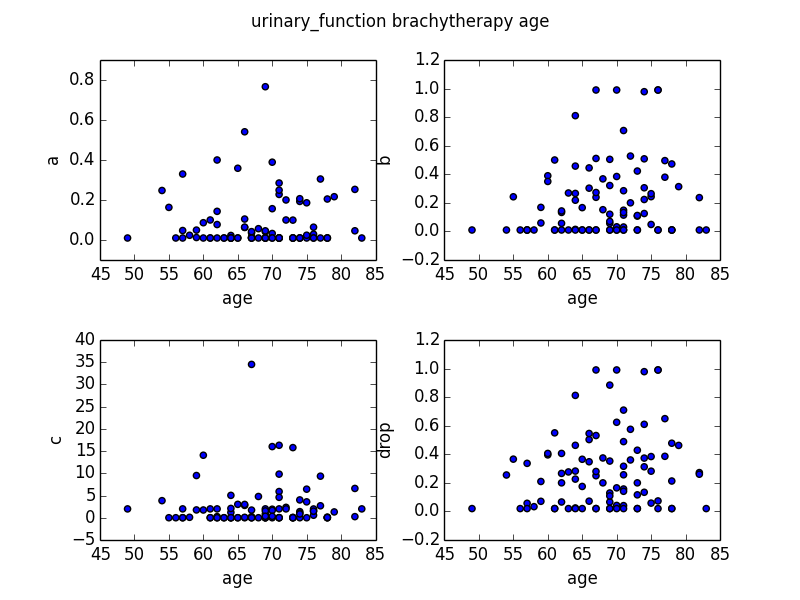
\includegraphics[width=.45\linewidth,height=0.3\textheight]{/Users/glareprotector/Documents/lab/glare/tex_files/sections/exploratory_with_abc/files/attribute_vs_curve_parameters/urinary_function_brachytherapy_age.png}}
\end{subfigure}
\caption{Urinary Function / Brachytherapy}
\end{figure}

\begin{figure}
\centering
\begin{subfigure}{
  \includegraphics[width=.45\linewidth,height=0.3\textheight]{/Users/glareprotector/Documents/lab/glare/prostate_code/files_for_rstan/bowel_function/surgery/B_abc_hist.png}}
\end{subfigure}
\begin{subfigure}{
  \includegraphics[width=.45\linewidth,height=0.3\textheight]{/Users/glareprotector/Documents/lab/glare/prostate_code/files_for_rstan/bowel_function/surgery/B_phi_hist.png}}
\end{subfigure}
\begin{subfigure}{
  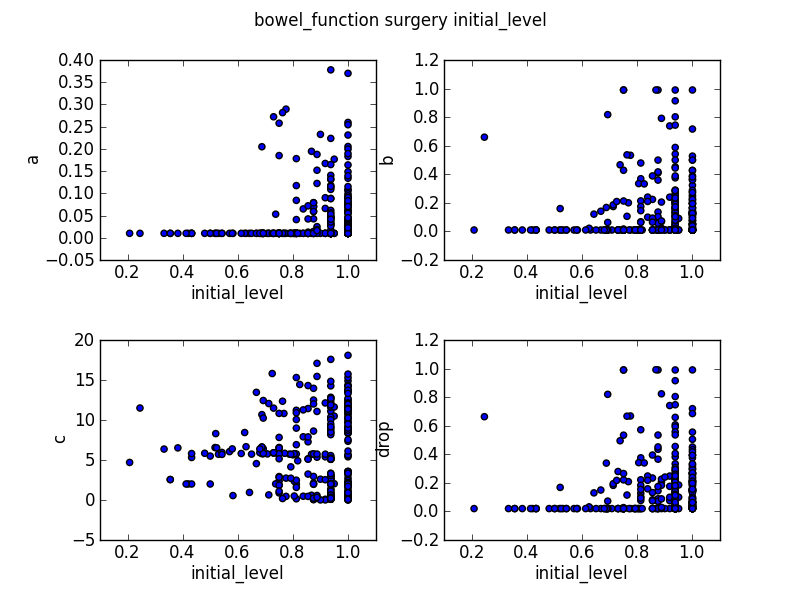
\includegraphics[width=.45\linewidth,height=0.3\textheight]{/Users/glareprotector/Documents/lab/glare/tex_files/sections/exploratory_with_abc/files/attribute_vs_curve_parameters/bowel_function_surgery_initial_level.png}}
\end{subfigure}
\begin{subfigure}{
  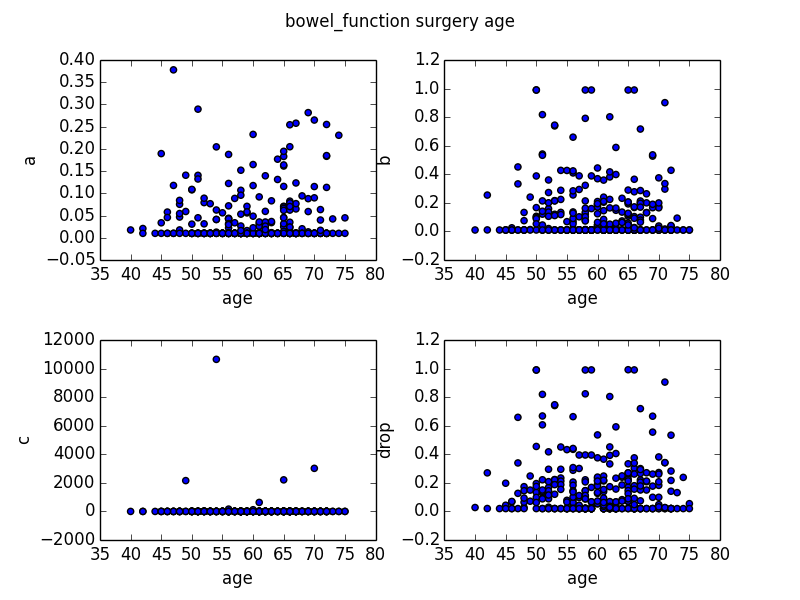
\includegraphics[width=.45\linewidth,height=0.3\textheight]{/Users/glareprotector/Documents/lab/glare/tex_files/sections/exploratory_with_abc/files/attribute_vs_curve_parameters/bowel_function_surgery_age.png}}
\end{subfigure}
\caption{Bowel Function / Surgery}
\end{figure}

\begin{figure}
\centering
\begin{subfigure}{
  \includegraphics[width=.45\linewidth,height=0.3\textheight]{/Users/glareprotector/Documents/lab/glare/prostate_code/files_for_rstan/bowel_function/radiation/B_abc_hist.png}}
\end{subfigure}
\begin{subfigure}{
  \includegraphics[width=.45\linewidth,height=0.3\textheight]{/Users/glareprotector/Documents/lab/glare/prostate_code/files_for_rstan/bowel_function/radiation/B_phi_hist.png}}
\end{subfigure}
\begin{subfigure}{
  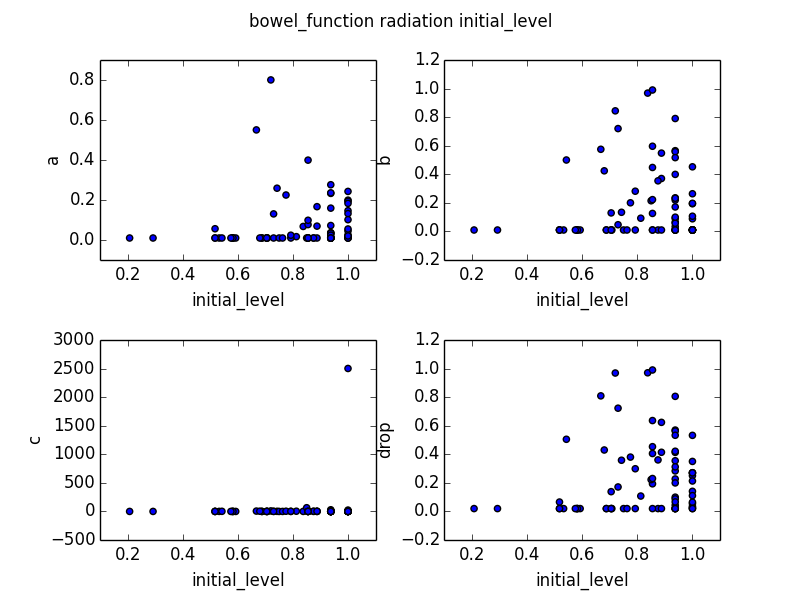
\includegraphics[width=.45\linewidth,height=0.3\textheight]{/Users/glareprotector/Documents/lab/glare/tex_files/sections/exploratory_with_abc/files/attribute_vs_curve_parameters/bowel_function_radiation_initial_level.png}}
\end{subfigure}
\begin{subfigure}{
  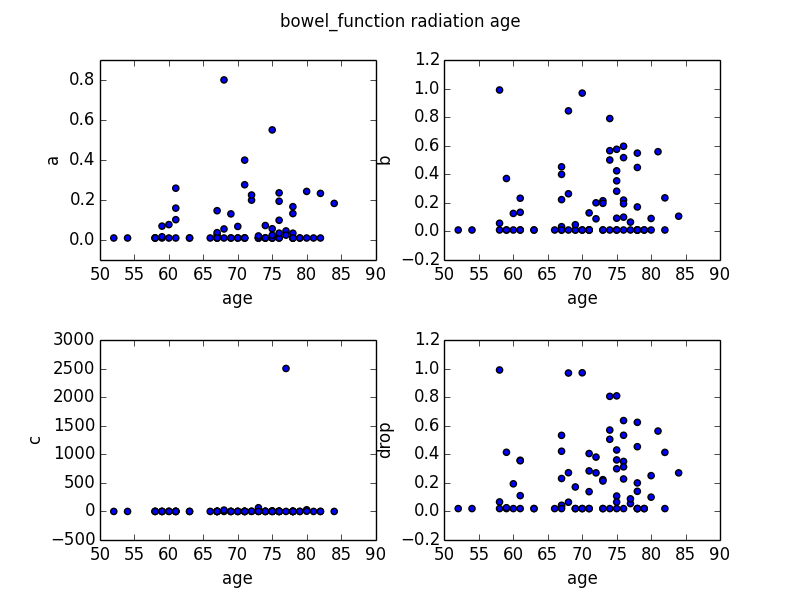
\includegraphics[width=.45\linewidth,height=0.3\textheight]{/Users/glareprotector/Documents/lab/glare/tex_files/sections/exploratory_with_abc/files/attribute_vs_curve_parameters/bowel_function_radiation_age.png}}
\end{subfigure}
\caption{Bowel Function / Radiation}
\end{figure}

\begin{figure}
\centering
\begin{subfigure}{
  \includegraphics[width=.45\linewidth,height=0.3\textheight]{/Users/glareprotector/Documents/lab/glare/prostate_code/files_for_rstan/bowel_function/brachytherapy/B_abc_hist.png}}
\end{subfigure}
\begin{subfigure}{
  \includegraphics[width=.45\linewidth,height=0.3\textheight]{/Users/glareprotector/Documents/lab/glare/prostate_code/files_for_rstan/bowel_function/brachytherapy/B_phi_hist.png}}
\end{subfigure}
\begin{subfigure}{
  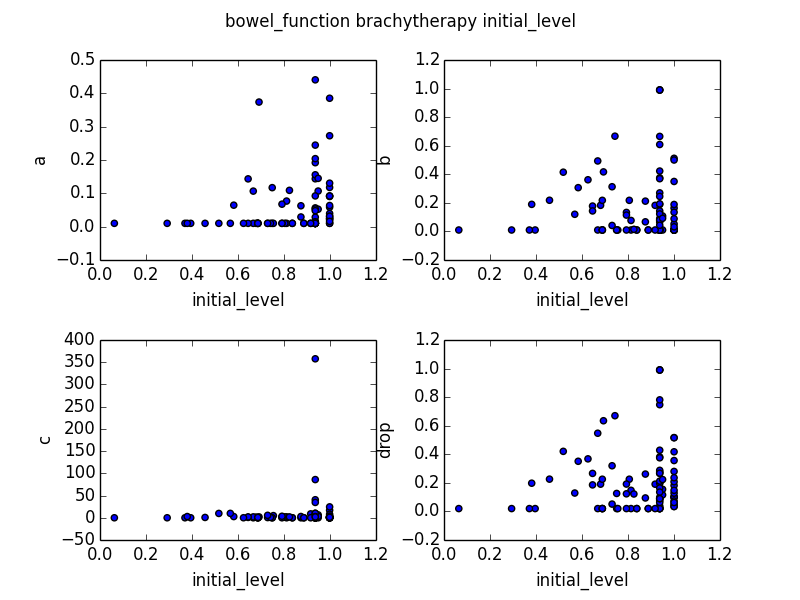
\includegraphics[width=.45\linewidth,height=0.3\textheight]{/Users/glareprotector/Documents/lab/glare/tex_files/sections/exploratory_with_abc/files/attribute_vs_curve_parameters/bowel_function_brachytherapy_initial_level.png}}
\end{subfigure}
\begin{subfigure}{
  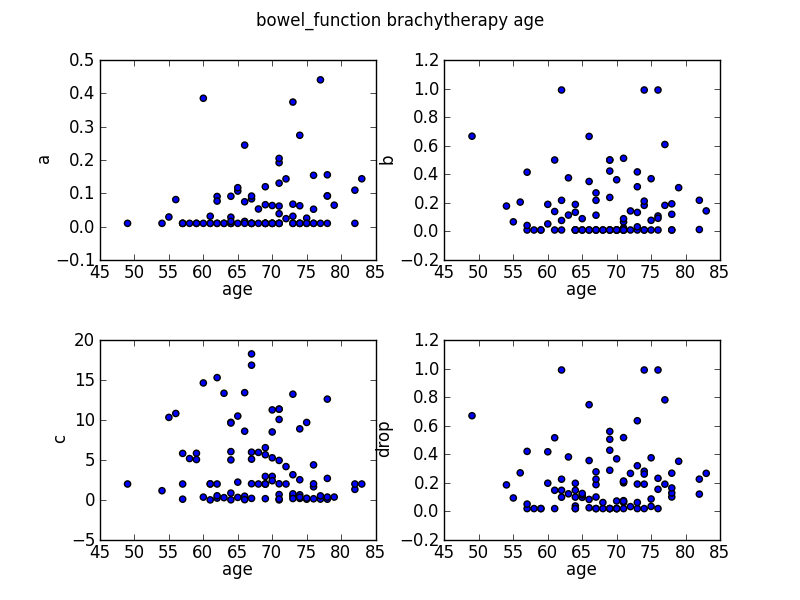
\includegraphics[width=.45\linewidth,height=0.3\textheight]{/Users/glareprotector/Documents/lab/glare/tex_files/sections/exploratory_with_abc/files/attribute_vs_curve_parameters/bowel_function_brachytherapy_age.png}}
\end{subfigure}
\caption{Bowel Function / Brachytherapy}
\end{figure}